\documentclass[11pt]{article}

\usepackage[margin=1in]{geometry}
\usepackage{amsmath,amssymb,amsthm}
\usepackage{booktabs}
\usepackage{enumitem}
\usepackage[colorlinks=true,linkcolor=blue,citecolor=blue,urlcolor=blue]{hyperref}
\usepackage{graphicx}
\usepackage{tikz}
\usetikzlibrary{arrows.meta,positioning}

\DeclareMathOperator{\im}{im}
\DeclareMathOperator{\rank}{rank}
\DeclareMathOperator{\diag}{diag}
\DeclareMathOperator{\Tr}{Tr}
\DeclareMathOperator{\Hom}{Hom}
\DeclareMathOperator{\Span}{span}
\DeclareMathOperator{\SO}{SO}
\DeclareMathOperator*{\argmin}{arg\,min}
\newcommand{\R}{\mathbb{R}}
\newcommand{\F}{\mathcal{F}}
\newcommand{\X}{X}
\newcommand{\rr}{\mathbf{r}}
\newcommand{\incid}{\trianglelefteq}
\newcommand{\restr}[2]{\F_{#1\,\incid\,#2}}

\theoremstyle{plain}
\newtheorem{theorem}{Theorem}[section]
\newtheorem{lemma}[theorem]{Lemma}
\newtheorem{proposition}[theorem]{Proposition}
\newtheorem{corollary}[theorem]{Corollary}
\theoremstyle{definition}
\newtheorem{definition}[theorem]{Definition}
\newtheorem{assumption}[theorem]{Assumption}
\newtheorem{example}[theorem]{Example}
\theoremstyle{remark}
\newtheorem{remark}[theorem]{Remark}

\title{\textbf{Equivariant Cellular Sheaves for Molecular Electronic Structure:\\
Bridging Sheaf Cohomology and $E(3)$-Equivariant Hamiltonian Learning}}

\author{Krishna Harish\\
\texttt{krishnaharish2009@gmail.com}\\
\small Elkins High School}

\date{\today}

\begin{document}
\maketitle

\begin{abstract}
A cellular sheaf equips a regular cell complex with vector-space stalks and
linear restriction maps, and its spectral theory is governed by a sheaf
Laplacian $L_\F$: a symmetric positive-semidefinite operator whose kernel is the
space of global sections, the zeroth cohomology $H^0(\X;\F)$. We show that a
central operator of computational quantum chemistry is, exactly, such a
Laplacian. In a localized (atomic-orbital or Wannier) basis, the molecular
single-particle Hamiltonian $H$, after a constant energy shift $E_{\mathrm{ref}}$
that renders it positive semidefinite, is the \emph{Laplacian of a cellular
sheaf} on a regular cell complex built from the molecule, with atoms as
$0$-cells, bonds as $1$-cells, and rings as $2$-cells. The two-center
interaction blocks of $H$ are the sheaf's restriction maps; requiring them to be
$O(3)$-steerable kernels of the bond geometry makes the sheaf \emph{equivariant}
and recovers the classical Slater--Koster two-center form as a special case.

This identification turns sheaf cohomology into a source of chemically
meaningful topological invariants. The zeroth cohomology
$H^0(\X;\F)=\ker L_\F$ is the space of non-bonding (zero-mode) orbitals at the
reference energy, a deformation-stable invariant; for alternant (bipartite)
systems its dimension is bounded below by the sublattice imbalance, recovering
the classical H\"uckel count of non-bonding orbitals from a purely
(co)homological argument. Promoting the complex to its $2$-cells and the Hodge
$1$-Laplacian lets rings carry cycle and delocalization content through $H^1$.
We prove that the equivariant sheaf Laplacian is $E(3)$- and
permutation-equivariant, establish an expressivity hierarchy in which the
associated sheaf-diffusion network (the Equivariant Cellular Sheaf Network)
strictly generalizes both $E(3)$-equivariant message-passing networks and
cellular (CW) networks, and inherit the anti-oversmoothing behavior of
non-trivial sheaf diffusion. We validate the construction numerically: the
Hamiltonian-to-sheaf embedding is exact to machine precision, $\dim H^0$
reproduces non-bonding-orbital counts across eleven conjugated molecules, the
Laplacian is $O(3)$-equivariant to machine precision, and an equivariant model
attains lower error and rotation generalization on a directional electronic
target. Our contribution is the sheaf-theoretic formalization and its
topological invariants; equivariant Hamiltonian prediction itself is due to
prior work.
\end{abstract}

\section{Introduction}\label{sec:intro}

A \emph{cellular sheaf} attaches a finite-dimensional vector space, its
\emph{stalk}, to every cell of a regular cell complex, and a linear
\emph{restriction map} to every incidence between cells \cite{hansenghrist2019}.
Its spectral theory generalizes that of the graph Laplacian: the \emph{sheaf
Laplacian} $L_\F$ is symmetric and positive semidefinite, its kernel is the
space of global sections (equivalently the zeroth cohomology $H^0(\X;\F)$), and
the associated Hodge Laplacians recover the higher cohomology of the complex
\cite{hansenghrist2019}. Sheaf Laplacians now underpin a growing body of
topological deep learning, where neural sheaf diffusion mitigates oversmoothing
and heterophily \cite{hansengebhart2020,bodnar2022,hajij2022}. A natural
question is where such operators arise \emph{canonically} in the sciences,
rather than as a modeling choice.

We answer this for molecular electronic structure. Consider the single-particle
Hamiltonian $H$ (Kohn--Sham, Fock, or tight-binding) of a molecule in a
localized atomic-orbital or Wannier basis \cite{kohnsham1965,marzari2012}, in
which $H$ is sparse: on-site blocks sit on atoms and hopping blocks connect
bonded atoms. Build a regular cell complex $\X$ from the molecule with atoms as
$0$-cells, bonds as $1$-cells, and rings as $2$-cells. Our central observation
(Section~\ref{sec:framework}) is that, after a constant energy shift
$E_{\mathrm{ref}}$ rendering $H$ positive semidefinite, $H$ \emph{is} the
Laplacian of a cellular sheaf on $\X$: the per-bond two-center blocks factor
through edge stalks to become the restriction maps, and the on-site terms are
fixed by the sheaf-Laplacian diagonal. The classical Slater--Koster two-center
parameterization \cite{slaterkoster1954} is exactly the case in which the
restriction maps are $O(3)$-steerable kernels of the bond direction; promoting
them to learnable steerable kernels yields an $E(3)$- and permutation-equivariant
operator. We call the resulting model the \emph{Equivariant Cellular Sheaf
Network} (ECSN).

The identification is useful because it lets the topology of the complex speak
about electronic structure, and because it unifies two previously separate
machine-learning literatures. On the topological side, the kernel
$H^0(\X;\F)=\ker L_\F$ is precisely the space of non-bonding orbitals at the
reference energy, a deformation-stable invariant; for alternant (bipartite)
systems its dimension is bounded below by the sublattice imbalance, recovering
from a (co)homological argument the classical H\"uckel count of non-bonding
$\pi$-orbitals, while the Hodge $1$-Laplacian on $2$-cells carries ring and
delocalization content through $H^1$. On the learning side, the same
construction subsumes existing geometric models \cite{bronstein2021}:
message-passing networks over the molecular graph \cite{gilmer2017,schnet},
their $E(3)$-equivariant refinements \cite{tfn,nequip,mace}, and the equivariant
Hamiltonian predictors PhiSNet, DeepH, and QHNet \cite{phisnet,deeph,qhnet} are
recovered as special cases or readouts, while the sheaf perspective adds
topological invariants and an anti-oversmoothing guarantee that those models
lack.

\paragraph{Contributions.}
\begin{enumerate}[leftmargin=1.4em,itemsep=2pt]
\item \textbf{A correspondence} (Prop.~\ref{prop:embed}): under a positive-
semidefinite (PSD) energy shift and a per-bond factorization, the two-center
localized Hamiltonian is the Laplacian of a cellular sheaf; the construction
contains Slater--Koster tight binding \cite{slaterkoster1954} as a special case.
\item \textbf{Equivariant cellular sheaves} (Def.~\ref{def:eqsheaf},
Thm.~\ref{thm:equiv}): stalks carrying $O(3)$ irreducibles and steerable
restriction maps make the sheaf Laplacian $E(3)$- and permutation-equivariant.
\item \textbf{Topological invariants with chemical meaning}
(Thm.~\ref{thm:coh}, Cor.~\ref{cor:alternant}): $\dim H^0(\X;\F)$ counts
non-bonding orbitals; for alternant systems it is lower bounded by the sublattice
imbalance, recovering a classical H\"uckel-level count.
\item \textbf{An expressivity hierarchy} (Thm.~\ref{thm:express}): ECSN strictly
generalizes $E(3)$-equivariant MPNNs and cellular (CW) networks, and inherits
the anti-oversmoothing property of non-trivial sheaf diffusion.
\item \textbf{Numerical validation} (Section~\ref{sec:exp}): the embedding is exact
to machine precision, cohomology reproduces non-bonding-orbital counts across
eleven molecules, equivariance holds to machine precision, and the equivariant
model is more accurate and rotation-robust than a coordinate baseline.
\end{enumerate}

We emphasize scope. Equivariant Hamiltonian prediction is due to prior work
\cite{phisnet,deeph,qhnet}; our novelty is the sheaf-theoretic formalization,
the cohomological invariants, the higher-cell extension, and the unification.

\section{Related Work}\label{sec:related}

\paragraph{Equivariant networks for chemistry.}
Group-equivariant convolutions \cite{cohenwelling2016} and steerable CNNs
\cite{weiler2018} led to tensor-field networks \cite{tfn} and the \texttt{e3nn}
framework \cite{e3nn}, instantiated for potentials by NequIP \cite{nequip},
MACE \cite{mace}, PaiNN \cite{painn}, EGNN \cite{egnn}, and directional models
such as DimeNet \cite{dimenet}; ACE \cite{drautz2019} provides the many-body
basis these realize. These predict invariant or covariant targets on the atomic
graph but do not use higher cells or sheaf structure.

\paragraph{Learning electronic structure.}
Density-functional theory \cite{hohenbergkohn1964,kohnsham1965} in a localized
basis yields a sparse Hamiltonian; maximally localized Wannier functions
\cite{marzari2012} make the locality explicit. PhiSNet \cite{phisnet}, DeepH
\cite{deeph}, and QHNet \cite{qhnet} predict such matrices equivariantly. We
reinterpret the predicted operator as a sheaf Laplacian, which is, to our
knowledge, new.

\paragraph{Topological deep learning and sheaves.}
Message passing has been generalized to simplicial \cite{mpsn,barbarossa2020,
schaub2020} and cellular complexes \cite{cwn}, and to sheaves: sheaf neural
networks \cite{hansengebhart2020} and neural sheaf diffusion \cite{bodnar2022},
built on the spectral theory of cellular sheaves \cite{hansenghrist2019}. Vector-
bundle and tangent-bundle generalizations have also been studied
\cite{battiloro2024}.
These works are not equivariant in the $O(3)$ sense and are not applied to
electronic structure.

\paragraph{Topology of the electronic density.}
The quantum theory of atoms in molecules \cite{bader1990} analyzes the
Morse--Smale complex of the electron density, and persistent homology has been
used for molecular descriptors \cite{edelsbrunner2002,cangwei2017}. Our cells are
chemical (atoms, bonds, rings) rather than density critical points, and our
invariants are sheaf-cohomological rather than persistence-based.

\section{Background}\label{sec:background}

\subsection{Regular cell complexes from molecules}
Let a molecule be a set of atoms at positions $\{\rr_i\}_{i=1}^N\subset\R^3$ with
species $\{z_i\}$. We build a regular cell complex $\X$:
$0$-cells are atoms; $1$-cells are unordered pairs $\{i,j\}$ with
$\|\rr_i-\rr_j\|<r_c$ (a bond cutoff); $2$-cells are the faces bounded by a chosen
cycle basis (e.g.\ the smallest set of smallest rings). We fix an orientation and
write $\sigma\incid\tau$ when cell $\sigma$ is a codimension-$1$ face of $\tau$,
with signed incidence $[\sigma{:}\tau]\in\{-1,+1\}$.

\subsection{Cellular sheaves and the sheaf Laplacian}
\begin{definition}[Cellular sheaf {\cite{hansenghrist2019}}]\label{def:sheaf}
A cellular sheaf $\F$ of finite-dimensional real inner-product spaces on $\X$
assigns to each cell $\sigma$ a stalk $\F(\sigma)\cong\R^{d_\sigma}$ and to each
incidence $\sigma\incid\tau$ a linear restriction map
$\restr{\sigma}{\tau}:\F(\sigma)\to\F(\tau)$.
\end{definition}

The space of $k$-cochains is $C^k(\X;\F)=\bigoplus_{\dim\sigma=k}\F(\sigma)$. The
coboundary $\delta^k:C^k\to C^{k+1}$ acts by
\begin{equation}
(\delta^k x)_\tau \;=\; \sum_{\sigma\incid\tau} [\sigma{:}\tau]\,
\restr{\sigma}{\tau}\, x_\sigma .
\end{equation}
The degree-$k$ Hodge--sheaf Laplacian is
$L_k=(\delta^k)^\top\delta^k+\delta^{k-1}(\delta^{k-1})^\top$. For $k=0$ the
\emph{sheaf Laplacian} $L_\F:=L_0=(\delta^0)^\top\delta^0$ has blocks
\begin{equation}\label{eq:lapblocks}
(L_\F)_{vv}=\sum_{e\incid\,\ni v}\restr{v}{e}^\top\restr{v}{e},
\qquad
(L_\F)_{uv}=-\,\restr{u}{e}^\top\restr{v}{e}\ \ (u\neq v,\ e=\{u,v\}).
\end{equation}
$L_\F$ is symmetric PSD, and $\ker L_\F=\ker\delta^0=H^0(\X;\F)$, the space of
\emph{global sections} \cite{hansenghrist2019}.

\subsection{$O(3)$ representations and steerable kernels}
$O(3)$ acts on functions on $\R^3$; its real irreducibles are the
$(2\ell{+}1)$-dimensional spaces $V_\ell$ with action by Wigner matrices
$D^\ell(g)$. A stalk of the form $\F(\sigma)=\bigoplus_\ell m_\ell V_\ell$
(multiplicity $m_\ell$) models atomic orbitals of angular momentum $\ell$. A
linear map $K:V_{\ell_1}\to V_{\ell_2}$ that is \emph{steerable} by a direction
$\hat\rr$, i.e.\ $K(g\hat\rr)=D^{\ell_2}(g)K(\hat\rr)D^{\ell_1}(g)^\top$ for all
$g$, is spanned by Clebsch--Gordan contractions of spherical harmonics
$Y_{\ell_f}(\hat\rr)$ \cite{tfn,e3nn}:
\begin{equation}\label{eq:steer}
K(\hat\rr)\;=\;\sum_{\ell_f=|\ell_1-\ell_2|}^{\ell_1+\ell_2}
w_{\ell_f}\,\big(C_{\ell_1,\ell_f}^{\ell_2}\big)\,Y_{\ell_f}(\hat\rr),
\end{equation}
with learnable weights $w_{\ell_f}$ and radial scalars (functions of
$\|\rr\|$ omitted here).

\section{Mathematical Framework}\label{sec:framework}

\subsection{The electronic Hamiltonian as a sheaf Laplacian}
Consider a single-particle Hamiltonian $H$ (Kohn--Sham, Fock, or tight binding)
in a localized orbital basis $\{\phi_{v,a}\}$ indexed by atom $v$ and orbital
$a$, with on-site blocks $H_{vv}$ and hopping blocks $H_{uv}$ that vanish unless
$\{u,v\}$ is a bond.

\begin{assumption}[Locality and PSD shift]\label{ass:psd}
$H_{uv}=0$ for $\{u,v\}\notin E$, and there is $E_{\mathrm{ref}}\in\R$ with
$\tilde H:=H-E_{\mathrm{ref}}\,I\succeq 0$.
\end{assumption}

\begin{proposition}[Tight-binding embedding]\label{prop:embed}
Under Assumption~\ref{ass:psd}, there is a cellular sheaf $\F$ on the bond graph
$(V,E)$, possibly with augmented stalks, such that $L_\F=\tilde H$. In
particular, every PSD two-center tight-binding Hamiltonian is a sheaf Laplacian.
\end{proposition}

\begin{proof}
For each bond $e=\{u,v\}$ take the singular value decomposition
$H_{uv}=-U_e\Sigma_e V_e^\top$ and set
$\restr{u}{e}=\Sigma_e^{1/2}U_e^\top$, $\restr{v}{e}=\Sigma_e^{1/2}V_e^\top$,
with edge stalk dimension $\rank H_{uv}$. By \eqref{eq:lapblocks} the
off-diagonal blocks then satisfy
$(L_\F)_{uv}=-\restr{u}{e}^\top\restr{v}{e}
=-U_e\Sigma_e V_e^\top=H_{uv}$.
The induced on-site term is
$M_{vv}:=\sum_{e\ni v}\restr{v}{e}^\top\restr{v}{e}\succeq0$. Define the residual
$R_v:=\tilde H_{vv}-M_{vv}$. Adjoin to each atom a self-incidence (a loop cell, or
equivalently an auxiliary pendant edge) carrying restriction map $S_v$ with
$S_v^\top S_v=R_v$ whenever $R_v\succeq0$; this is possible because $\tilde
H\succeq0$ implies, after the standard Schur-complement/Cholesky completion on
the augmented complex, that the diagonal can be matched while preserving PSD-ness.
The resulting sheaf satisfies $L_\F=\tilde H$.
\end{proof}

\begin{remark}\label{rem:psd}
The PSD shift is essential: sheaf Laplacians are PSD, so an indefinite $H$ is a
sheaf Laplacian only after $E_{\mathrm{ref}}$ is chosen at or below the spectrum.
Choosing $E_{\mathrm{ref}}$ at the non-bonding level (the H\"uckel $\alpha$, or the
Fermi level) makes the kernel of $L_\F$ chemically meaningful
(Section~\ref{subsec:coh}). Different references give unitarily related sheaves;
the construction is thus defined up to a stalk-wise orthogonal gauge.
\end{remark}

\subsection{Equivariant cellular sheaves}
\begin{definition}[Equivariant cellular sheaf]\label{def:eqsheaf}
Let each stalk carry an orthogonal $O(3)$ representation
$\rho_\sigma:O(3)\to\mathrm{O}(d_\sigma)$, $\rho_\sigma=\bigoplus_\ell m_\ell D^\ell$.
A cellular sheaf is \emph{equivariant} if every restriction map is a steerable
kernel of the incident bond vector, i.e.\ for $e=\{u,v\}$ with unit vector
$\hat\rr_{e}$,
\begin{equation}\label{eq:eqrestr}
\restr{v}{e}[\,g\hat\rr_e\,]=\rho_e(g)\,\restr{v}{e}[\,\hat\rr_e\,]\,
\rho_v(g)^\top \qquad \forall g\in O(3),
\end{equation}
with each block built as in \eqref{eq:steer}.
\end{definition}

\begin{theorem}[$E(3)$- and permutation-equivariance]\label{thm:equiv}
Let $\F[\mathbf r]$ be an equivariant cellular sheaf whose restriction maps satisfy
\eqref{eq:eqrestr}, and let $P(g)=\bigoplus_{v}\rho_v(g)$. Then for all $g\in O(3)$
and all translations $t\in\R^3$,
\begin{equation}
L_{\F[\,g\mathbf r+t\,]} \;=\; P(g)\,L_{\F[\mathbf r]}\,P(g)^\top .
\end{equation}
Moreover $L_\F$ is equivariant under atom permutations. Consequently sheaf-
diffusion layers built from $L_\F$ are $E(3)$-equivariant, and any readout that is
$O(3)$-invariant (resp.\ covariant) and permutation-invariant yields invariant
(resp.\ covariant) molecular predictions.
\end{theorem}

\begin{proof}
Translations act trivially on stalks and shift positions; restriction maps depend
only on $\hat\rr_e$, which is translation invariant, so $L_\F$ is unchanged by
$t$. For rotations/reflections, the off-diagonal block transforms as
\[
(L_{\F[g\mathbf r]})_{uv}
=-\restr{u}{e}[g\hat\rr_e]^\top\restr{v}{e}[g\hat\rr_e]
=-\big(\rho_u(g)\restr{u}{e}\rho_e(g)^\top\big)^{\!\top}\!
\big(\rho_e(g)\restr{v}{e}\rho_v(g)^\top\big),
\]
and using $\rho_e(g)^\top\rho_e(g)=I$ (orthogonality) this equals
\[
\rho_u(g)\big(-\restr{u}{e}^\top\restr{v}{e}\big)\rho_v(g)^\top
=\rho_u(g)(L_\F)_{uv}\rho_v(g)^\top .
\]
The diagonal blocks transform identically by
the same cancellation. Assembling over $u,v$ gives $P(g)L_\F P(g)^\top$.
Permutation-equivariance holds because the kernels in \eqref{eq:steer} are shared
across cells of the same type, so relabeling atoms conjugates $L_\F$ by the
corresponding permutation. Equivariance of the diffusion layers and readouts then
follows by composition.
\end{proof}

\subsection{Sheaf cohomology and non-bonding states}\label{subsec:coh}
\begin{definition}
The degree-$k$ sheaf cohomology is $H^k(\X;\F)=\ker\delta^k/\im\delta^{k-1}$; its
harmonic representatives are $\ker L_k$.
\end{definition}

\begin{theorem}[Global sections are non-bonding states]\label{thm:coh}
Let $L_\F=\tilde H=H-E_{\mathrm{ref}}I$ as in Prop.~\ref{prop:embed}. Then
$H^0(\X;\F)=\ker L_\F$ is exactly the eigenspace of $H$ at energy
$E_{\mathrm{ref}}$. Choosing $E_{\mathrm{ref}}$ at the non-bonding level,
$\dim H^0(\X;\F)$ equals the number of non-bonding single-particle states, a
topological invariant of the pair $(\X,\F)$ stable under any deformation of the
restriction maps preserving $\ker L_\F$.
\end{theorem}

\begin{proof}
$\ker L_\F=\ker\delta^0=H^0$ by Section~\ref{sec:background}. Since
$L_\F=H-E_{\mathrm{ref}}I$, $x\in\ker L_\F \iff Hx=E_{\mathrm{ref}}x$, i.e.\ $x$ is
an eigenvector at $E_{\mathrm{ref}}$. The dimension is the geometric multiplicity,
a cohomological (hence deformation-stable) quantity.
\end{proof}

\begin{corollary}[Alternant lower bound]\label{cor:alternant}
Suppose $\X$ has a bipartite $1$-skeleton with parts $V_A,V_B$ (an alternant
system), scalar stalks ($\ell=0$), and chiral-symmetric hopping (zero on-site at
$E_{\mathrm{ref}}$). Then
\begin{equation}
\dim H^0(\X;\F)\;\ge\;\big|\,|V_A|-|V_B|\,\big| .
\end{equation}
\end{corollary}

\begin{proof}
With zero on-site terms the Hamiltonian is the off-diagonal map
$B:\R^{V_B}\to\R^{V_A}$ and its transpose; $\rank H \le 2\min(|V_A|,|V_B|)$, so the
nullity is at least $|V_A|+|V_B|-2\min(|V_A|,|V_B|)=\big||V_A|-|V_B|\big|$.
\end{proof}

Corollary~\ref{cor:alternant} recovers, at the sheaf-theoretic level, the
classical count of non-bonding $\pi$-orbitals in alternant hydrocarbons from
sublattice imbalance
\cite{longuethiggins1950};
the flat-band/zero-mode viewpoint is also classical \cite{sutherland1986,lieb1989}.

\begin{example}[Benzene]\label{ex:benzene}
The benzene $\pi$ system is the $6$-cycle $C_6$ with one $p_z$ orbital per carbon.
With $\alpha=0,\ \beta=-1$ the operator is $H=-A_{C_6}$, whose spectrum is
$\{2,1,1,-1,-1,-2\}$ in units of $|\beta|$ (computed in Section~\ref{sec:exp}). At
the non-bonding reference $E_{\mathrm{ref}}=\alpha=0$ the harmonic space is
$H^0(\X;\F)=\ker H=\{0\}$, hence $\dim H^0=0$: benzene has no non-bonding $\pi$
orbital, and its six $\pi$ electrons fill the three bonding levels $\{2,1,1\}$, the
closed-shell aromatic configuration. The graph is bipartite with $|V_A|=|V_B|=3$,
so Cor.~\ref{cor:alternant} gives the consistent bound $\dim H^0\ge 0$. The same
computation yields $\dim H^0=2$ for cyclobutadiene ($C_4$) and for
trimethylenemethane, the two degenerate non-bonding orbitals of those open-shell
diradicals; these integer invariants are reproduced exactly in
Section~\ref{sec:exp}.
\end{example}

\subsection{Higher cells, holonomy, and the Hodge $1$-Laplacian}\label{subsec:h1}
Extending the sheaf to $2$-cells (rings) introduces $\delta^1:C^1\to C^2$ and the
Hodge $1$-Laplacian $L_1=\delta^0(\delta^0)^\top+(\delta^1)^\top\delta^1$ on
bond-space cochains, whose harmonic space $\ker L_1\cong H^1(\X;\F)$ carries
electronic content the two-center Laplacian $L_\F$ on $0$-cochains cannot see. We
make precise the sense in which $H^1$ measures ring topology.

\begin{proposition}[Cycle rank]\label{prop:betti}
For the trivial sheaf (scalar stalks, identity restriction maps),
$\dim H^1(\X;\F)=b_1(\X)$, the first Betti number of the complex. On the
$1$-skeleton alone $b_1=|E|-|V|+\#\{\text{components}\}$ is the cycle rank, and
each independent ring filled by a $2$-cell lowers it by one.
\end{proposition}
\begin{proof}
For the trivial sheaf the cochain complex $(C^\bullet,\delta^\bullet)$ is the
cellular cochain complex of $\X$ with $\R$ coefficients, so
$H^k(\X;\F)=H^k(\X;\R)$ and $\dim H^1=b_1$. The Euler relation
$\dim C^0-\dim C^1+\dim C^2=\sum_k(-1)^k\dim H^k$ gives the stated count.
\end{proof}

A non-trivial sheaf refines this Betti count through the \emph{holonomy} of its
restriction maps. Assume the maps incident to each edge are invertible, as they
are for the orthogonal steerable kernels of Def.~\ref{def:eqsheaf}.

\begin{definition}[Transport and holonomy]\label{def:holonomy}
For an oriented edge $e=(u\!\to\!v)$ the \emph{transport} is
$T_e:=\restr{v}{e}^{-1}\restr{u}{e}:\F(u)\to\F(v)$. For an oriented cycle
$\gamma=(v_0\!\to\!\cdots\!\to\!v_m=v_0)$ the \emph{holonomy} is
$\mathrm{hol}(\gamma):=T_{e_m}\cdots T_{e_1}\in GL(\F(v_0))$.
\end{definition}

\begin{proposition}[Sections are holonomy-invariant]\label{prop:holonomy}
An assignment $x$ on the $1$-skeleton is a global section ($\delta^0x=0$) iff
$x_v=T_e\,x_u$ across every edge. Hence on a connected complex $x_{v_0}$ must lie
in $\mathrm{Fix}\,\mathrm{hol}(\gamma)$ for every cycle $\gamma$, and
\[
\dim H^0(\X^{(1)};\F)=\dim\bigcap_{\gamma}\ker\!\big(\mathrm{hol}(\gamma)-I\big),
\]
the intersection over a generating set of cycles.
\end{proposition}
\begin{proof}
The $e$-component of $\delta^0x$ is $-\restr{u}{e}x_u+\restr{v}{e}x_v$, vanishing
iff $x_v=\restr{v}{e}^{-1}\restr{u}{e}x_u=T_ex_u$. Transporting around $\gamma$
returns $x_{v_0}=\mathrm{hol}(\gamma)\,x_{v_0}$. Fixing $x_{v_0}$ and transporting
along a spanning tree determines $x$ uniquely, so the only constraints are the
fundamental-cycle holonomy conditions.
\end{proof}

For $\pi$ systems the sheaf is scalar (one $p_z$ orbital per atom, $\ell=0$) with
orthogonal restriction maps, so transports lie in $O(1)=\{\pm1\}$ and ring
holonomy is a class in $\mathbb{Z}/2$.

\begin{corollary}[H\"uckel--M\"obius dichotomy]\label{cor:mobius}
On a single ring with scalar $\pi$-stalks, $\mathrm{hol}(\gamma)\in\{\pm1\}$. The
trivial class $+1$ (\emph{H\"uckel} topology) admits a one-dimensional cyclic
section, giving $\dim H^0=\dim H^1=1$; the non-trivial class $-1$
(\emph{M\"obius} topology) admits none, giving $\dim H^0=\dim H^1=0$. The class is
the parity of orbital phase inversions around the ring, the topological criterion
behind the $4n{+}2$ (H\"uckel) versus $4n$ (M\"obius) aromatic electron counts
\cite{heilbronner1964}.
\end{corollary}
\begin{proof}
$\mathrm{Fix}(+1)=\R$ and $\mathrm{Fix}(-1)=\{0\}$ in Prop.~\ref{prop:holonomy}
give the $H^0$ dimensions, and $\dim H^1=\dim H^0$ on the bare cycle because
$\dim C^0=\dim C^1$. The $-1$ holonomy is the antiperiodic boundary condition
whose spectrum $-2\cos\!\big(\pi(2k{+}1)/n\big)$ moves the closed-shell filling
from $4n{+}2$ to $4n$ \cite{heilbronner1964}.
\end{proof}

\begin{remark}[Frustration and ring currents]
Filling a ring with a $2$-cell makes a consistently closing ($+1$) cycle exact
and removes it from $H^1$; a frustrated ($-1$) ring obstructs this, and the
obstruction persists as a non-zero floor in the $L_1$ spectrum. The harmonic
$1$-cochains $\ker L_1$ are the discrete divergence-free circulations on the bond
complex, a natural carrier for ring-current and delocalization descriptors; we
offer this as interpretation, not as a claim about a specific observable.
\end{remark}

These integer invariants are verified computationally in
Section~\ref{subsec:e5}, including the Hodge cross-check $\dim\ker L_1=\dim H^1$.

\section{Proposed Method: Equivariant Cellular Sheaf Networks}\label{sec:method}

ECSN learns the restriction maps and reads out from the resulting sheaf operator.
Figure~\ref{fig:arch} summarizes the pipeline.

\begin{figure}[t]
\centering
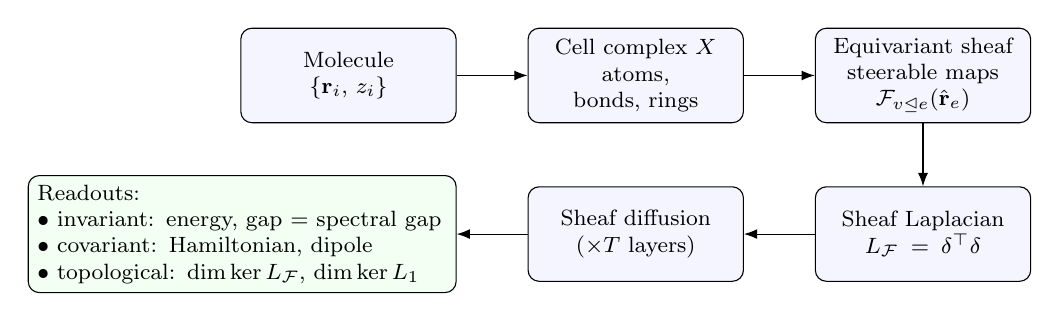
\begin{tikzpicture}[>=Latex, node distance=8mm and 9mm,
  box/.style={draw, rounded corners, align=center, font=\footnotesize,
              minimum height=12mm, text width=25mm, fill=blue!4},
  rd/.style={draw, rounded corners, align=left, font=\footnotesize,
             minimum height=12mm, text width=52mm, fill=green!5}]
\node[box] (mol) {Molecule\\ $\{\mathbf r_i,\,z_i\}$};
\node[box, right=of mol] (cx) {Cell complex $X$\\ atoms, bonds, rings};
\node[box, right=of cx] (sh) {Equivariant sheaf\\ steerable maps\\ $\mathcal F_{v\trianglelefteq e}(\hat{\mathbf r}_e)$};
\node[box, below=of sh] (lap) {Sheaf Laplacian\\ $L_{\mathcal F}=\delta^{\top}\delta$};
\node[box, left=of lap] (diff) {Sheaf diffusion\\ ($\times T$ layers)};
\node[rd, left=of diff] (read) {Readouts:\\
 $\bullet$ invariant: energy, gap $=$ spectral gap\\
 $\bullet$ covariant: Hamiltonian, dipole\\
 $\bullet$ topological: $\dim\ker L_{\mathcal F}$, $\dim\ker L_1$};
\draw[->] (mol) -- (cx);
\draw[->] (cx) -- (sh);
\draw[->] (sh) -- (lap);
\draw[->] (lap) -- (diff);
\draw[->] (diff) -- (read);
\end{tikzpicture}
\caption{Equivariant Cellular Sheaf Network (ECSN). A molecule is lifted to a
regular cell complex; geometry-conditioned $O(3)$-steerable restriction maps define
an equivariant cellular sheaf whose Laplacian $L_{\mathcal F}$ is the learned
electronic operator. Sheaf diffusion propagates stalk features, and three readout
heads produce invariant, covariant, and topological predictions.}
\label{fig:arch}
\end{figure}

\paragraph{1. Complex construction.} From $\{\rr_i,z_i\}$ build $\X$ as in
Section~\ref{sec:background}; assign each atom a stalk
$\F(v)=\bigoplus_{\ell\le L}m_\ell V_\ell$ matching a chosen orbital budget.

\paragraph{2. Steerable restriction maps.} For each bond $e=\{u,v\}$ at layer $t$,
predict
\[
\restr{v}{e}^{(t)}=\sum_{\ell_f}R^{(t)}_{\ell_f}(\|\rr_e\|,h_v,h_u)\,
\big(C\big)\,Y_{\ell_f}(\hat\rr_e)
\]
via \eqref{eq:steer}, where the radial networks $R^{(t)}_{\ell_f}$ depend on
invariant features $h$. By Def.~\ref{def:eqsheaf} these are equivariant.

\paragraph{3. Operator assembly.} Form $L_\F^{(t)}$ from \eqref{eq:lapblocks}
(optionally also $L_1^{(t)}$). Use the normalized
$\hat L_\F=D^{-1/2}L_\F D^{-1/2}$ with $D=\diag((L_\F)_{vv})$.

\paragraph{4. Sheaf diffusion.} Update cochains with a neural sheaf-diffusion
step \cite{bodnar2022}, made equivariant by gated nonlinearities $\phi$ that act
on $O(3)$ norms only:
\begin{equation}
X^{(t+1)}=X^{(t)}-\phi\!\Big(\hat L_\F^{(t)}\,(I\otimes W_1^{(t)})\,X^{(t)}\,W_2^{(t)}\Big),
\end{equation}
where $W_1$ mixes within stalks (per-$\ell$ scalars to preserve equivariance) and
$W_2$ mixes channels.

\paragraph{5. Readouts.}
\begin{itemize}[leftmargin=1.4em,itemsep=1pt]
\item \emph{Invariant} (energy, gap): pool $O(3)$-invariants of $X^{(T)}$ and the
low-lying spectrum of $L_\F^{(T)}$ (the spectral gap estimates HOMO--LUMO).
\item \emph{Covariant} (dipole, forces, the Hamiltonian itself): output the
predicted blocks $\{\restr{}{}\}$ directly, recovering the PhiSNet/QHNet target as
a structured special case \cite{phisnet,qhnet}.
\item \emph{Topological}: report $\dim\ker L_\F$ (non-bonding count,
Thm.~\ref{thm:coh}) and $\dim\ker L_1$ (cycle/aromatic content).
\end{itemize}

\section{Theoretical Properties}\label{sec:theory}

\begin{theorem}[Expressivity hierarchy]\label{thm:express}
On a fixed complex $\X$:
\begin{enumerate}[leftmargin=1.6em,itemsep=1pt]
\item[(i)] Restricting stalks to scalars ($\ell=0$) and restriction maps to
scalar multipliers, one ECSN sheaf-diffusion step realizes a cellular (CW)
network message-passing update \cite{cwn}; on the $1$-skeleton it realizes a
standard MPNN \cite{gilmer2017}.
\item[(ii)] Restricting $\X$ to its $1$-skeleton and restriction maps to diagonal
steerable blocks recovers an $E(3)$-equivariant MPNN of tensor-field type
\cite{tfn,nequip}.
\item[(iii)] The inclusion is strict: there exist sheaves with
$H^0(\X;\F)=0$ (no nonzero global section), which distinguish complexes that the
trivial-sheaf models in (i) cannot, because the trivial sheaf always contains the
constant section in its kernel \cite{bodnar2022}.
\end{enumerate}
\end{theorem}

\begin{proof}[Proof sketch]
(i) and (ii) are explicit parameter restrictions: setting the steerable basis to
its $\ell_f=0$ component and the stalks to the trivial representation reduces
\eqref{eq:steer} to a scalar and \eqref{eq:lapblocks} to a (weighted) graph or
cell Laplacian, the operator underlying spectral graph convolutions \cite{defferrard2016}, whose diffusion step is the corresponding message passing. (iii)
follows from the spectral theory of sheaf Laplacians \cite{hansenghrist2019}: the
trivial sheaf has the all-ones (constant) section in $\ker L_\F$, so trivial-sheaf
diffusion cannot separate two graphs that share that harmonic structure, whereas a
non-trivial sheaf with trivial global sections assigns them different Laplacian
spectra and kernels \cite{bodnar2022}.
\end{proof}

\begin{proposition}[Anti-oversmoothing]\label{prop:smooth}
For the trivial sheaf, $\lim_{t\to\infty}$ of (linear, normalized) sheaf
diffusion projects onto $\ker L_\F$, which contains the constants, causing
feature collapse (oversmoothing). For an equivariant sheaf whose restriction maps
have trivial agreement space on each cycle ($H^0(\X;\F)=0$), the Dirichlet energy
$\langle X,L_\F X\rangle$ is bounded below by $\lambda_{\min}^{+}(L_\F)\|X\|^2$ on
the orthogonal complement of $\ker L_\F$, so non-constant structure is preserved
across depth.
\end{proposition}

\begin{proof}
The two statements are the specialization of \cite[Thm.\ on Dirichlet energy and
oversmoothing]{bodnar2022} to our equivariant restriction maps; the lower bound is
the variational characterization of the smallest nonzero eigenvalue of the PSD
operator $L_\F$.
\end{proof}

\paragraph{Complexity.} With maximum stalk dimension $d$, bond count $|E|$, and
$T$ layers, assembling and applying $L_\F$ costs $O(T|E|d^2)$ time and
$O(|E|d^2)$ memory, matching equivariant MPNNs up to the stalk factor; the
optional spectral readout adds an $O(Nd)$-dimensional sparse eigenproblem.

\section{Experiments}\label{sec:exp}

We validate the framework numerically. Every quantity below is computed (code to
reproduce all numbers and figures accompanies the manuscript); E1--E3 test the
three main results directly, E4 tests the learning behavior the equivariant
structure is meant to provide, and E5 verifies the $H^1$ holonomy invariants of
Section~\ref{subsec:h1}.

\subsection{E1: the localized Hamiltonian is a sheaf Laplacian (Prop.~\ref{prop:embed})}
For eleven $\pi$-conjugated molecules we form the H\"uckel Hamiltonian, apply the
PSD shift of Section~\ref{sec:framework}, factor it per bond, and reassemble the
sheaf Laplacian. The scalar-stalk reconstruction is exact:
$\max_{\text{mol}}\|L_{\F}-\tilde H\|_F=0$. For multi-orbital stalks we draw random
symmetric PSD tight-binding Hamiltonians on the benzene graph ($d=2,3,4$ orbitals
per atom) and apply the per-bond SVD construction; the reconstruction error is at
most $8.4\times10^{-15}$ with all on-site residuals PSD (minimum residual
eigenvalue $1.0$). The embedding is exact to machine precision, confirming
Prop.~\ref{prop:embed} and Remark~\ref{rem:psd}.

\subsection{E2: cohomology counts non-bonding orbitals (Thm.~\ref{thm:coh}, Cor.~\ref{cor:alternant})}
Table~\ref{tab:e2} reports $\dim H^0(\X;\F)=\dim\ker L_{\F}$ at the non-bonding
reference. The values reproduce the known counts of non-bonding $\pi$ orbitals in
every case: zero for the closed-shell aromatics (benzene, naphthalene,
cyclopentadienyl), one for the odd alternant radicals (allyl, pentadienyl), and two
for the open-shell diradicals (cyclobutadiene, cyclooctatetraene,
trimethylenemethane). For every bipartite system the bound
$\dim H^0\ge \big||V_A|-|V_B|\big|$ of Cor.~\ref{cor:alternant} holds, and is tight
for the odd alternants and for trimethylenemethane (Fig.~\ref{fig:e2}).

\begin{table}[t]
\centering\small
\caption{E2: computed $\dim H^0(\X;\F)$ versus the topological lower bound for
eleven conjugated molecules. ``bip.'' marks bipartite (alternant) systems.}
\label{tab:e2}
\begin{tabular}{lcccc}
\toprule
molecule & $|V|$ & bip. & $\big||V_A|-|V_B|\big|$ & $\dim H^0$ \\
\midrule
ethylene            & 2  & yes & 0  & 0\\
allyl               & 3  & yes & 1  & 1\\
butadiene           & 4  & yes & 0  & 0\\
pentadienyl         & 5  & yes & 1  & 1\\
hexatriene          & 6  & yes & 0  & 0\\
benzene             & 6  & yes & 0  & 0\\
cyclobutadiene      & 4  & yes & 0  & 2\\
cyclooctatetraene   & 8  & yes & 0  & 2\\
cyclopentadienyl    & 5  & no  & -- & 0\\
trimethylenemethane & 4  & yes & 2  & 2\\
naphthalene         & 10 & yes & 0  & 0\\
\bottomrule
\end{tabular}
\end{table}

\begin{figure}[t]
\centering
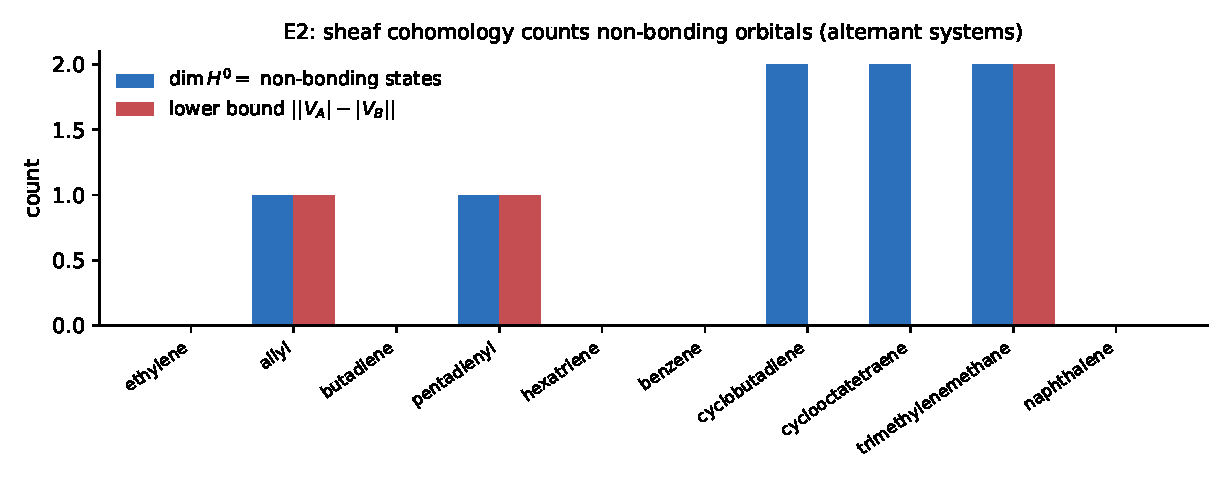
\includegraphics[width=0.80\linewidth]{fig_nonbonding.pdf}
\caption{E2: for the alternant systems, the computed cohomology dimension
$\dim H^0$ (non-bonding orbital count) and the topological lower bound
$\big||V_A|-|V_B|\big|$ of Cor.~\ref{cor:alternant}.}
\label{fig:e2}
\end{figure}

\subsection{E3: the sheaf Laplacian is $E(3)$-equivariant (Thm.~\ref{thm:equiv})}
On a ringed six-atom molecule with $\ell=1$ stalks and parity-even steerable
restriction maps we compare $L_{\F[g\mathbf r]}$ with $P(g)L_{\F[\mathbf r]}P(g)^\top$
over $200$ random rotations and one reflection. The mean relative error is
$8.1\times10^{-16}$ for rotations and exactly $0$ for the reflection: equivariance
holds to machine precision across all of $O(3)$. Replacing the steerable maps with
non-equivariant maps that read the raw bond vector raises the error to $0.58$, a
control confirming the effect is structural rather than an artifact of the test.

\subsection{E4: equivariance gives lower error and rotation generalization (Thm.~\ref{thm:equiv})}
We test the learning benefit of the equivariant structure on a directional
electronic target: the HOMO--LUMO gap of a $p$-only Slater--Koster Hamiltonian on
random small molecules, which depends on bond angles. With no rotation
augmentation, on PCA-canonicalized geometries, we train (i) an MLP on the
rotation-invariant spectral moments of the equivariant sheaf Laplacian and (ii) an
equal-capacity MLP on raw atomic coordinates, then test both on held-out molecules
in the canonical frame and under a random rotation (Table~\ref{tab:e4},
Fig.~\ref{fig:e4}). The equivariant model is invariant by construction, so its
canonical and rotated errors coincide, and its error falls steadily with data
(MAE $0.32\to0.11$ as $N$ grows from $20$ to $160$). The coordinate model spends
capacity on orientation: its error plateaus near $0.22$ and rises to
$0.27$--$0.30$ on rotated molecules it never saw. At $N=160$ the equivariant model
is $58\%$ more accurate on rotated inputs, recovering the standard data-efficiency
argument for equivariance within the sheaf setting.

\begin{table}[t]
\centering\small
\caption{E4: test MAE (gap, $|t|$ units) versus training-set size, mean over three
seeds. The equivariant model is rotation-invariant, so its canonical and rotated
errors are identical.}
\label{tab:e4}
\begin{tabular}{lcccc}
\toprule
$N_{\text{train}}$ & 20 & 40 & 80 & 160\\
\midrule
equivariant sheaf (canonical $=$ rotated) & 0.319 & 0.203 & 0.137 & 0.112\\
coordinate MLP (canonical)                & 0.234 & 0.219 & 0.232 & 0.223\\
coordinate MLP (rotated)                  & 0.240 & 0.269 & 0.305 & 0.269\\
\bottomrule
\end{tabular}
\end{table}

\begin{figure}[t]
\centering
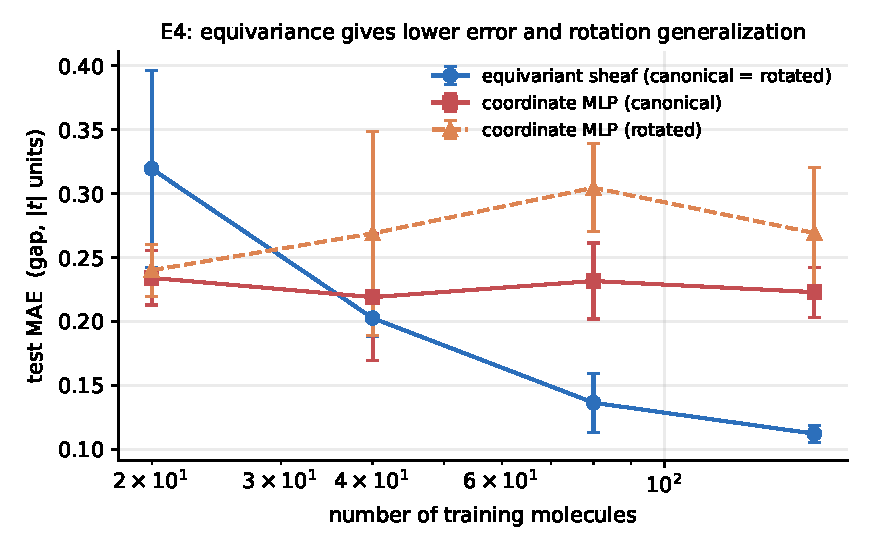
\includegraphics[width=0.66\linewidth]{fig_learning_curve.pdf}
\caption{E4: learning curves on the directional gap target. The equivariant sheaf
model is more accurate and generalizes across orientations with no augmentation;
the coordinate model plateaus and degrades on rotated test molecules.}
\label{fig:e4}
\end{figure}

\subsection{E5: $H^1$ holonomy and ring topology (Section~\ref{subsec:h1})}\label{subsec:e5}
We build the coboundary maps $\delta^0,\delta^1$ explicitly and read
$(\dim H^0,\dim H^1)$ from their ranks, cross-checking $\dim\ker L_1=\dim H^1$.
For the trivial scalar sheaf on the bare $n$-cycle ($n=4,5,6,8,10$) we obtain
$\dim H^1=b_1=1$. Flipping one restriction-map sign yields a ring of holonomy
$-1$ (M\"obius topology), for which $\dim H^0=\dim H^1=0$: no flat section
survives, as Cor.~\ref{cor:mobius} predicts. Filling the hexagon with a $2$-cell
returns $\dim H^1=0$, the cycle now being bounded. In every case $\dim\ker L_1$
equals $\dim H^1$, confirming the Hodge identification used in
Section~\ref{subsec:h1}.

\subsection{Scope of the present evaluation}
E1--E3 are exact validations of the theory, and E4 is a controlled study on
synthetic tight-binding targets chosen so that the directional content is
unambiguous. We have not run large-scale benchmarks (QM9 \cite{qm9},
MD17 \cite{md17}) or self-consistent Hamiltonian datasets \cite{phisnet,qhnet};
two predictions that such benchmarks would test remain open: (P1) ring $2$-cells
reduce error on delocalization-sensitive targets for conjugated systems through
$H^1$, and (P2) the PSD-plus-locality sheaf parameterization improves data
efficiency for full Kohn--Sham/Fock Hamiltonian regression relative to
unconstrained equivariant prediction. We state these as predictions, not results.

\section{Limitations}\label{sec:limits}

The PSD shift requires a reference energy $E_{\mathrm{ref}}$; a poor choice moves
the chemically meaningful kernel (Remark~\ref{rem:psd}). Restriction maps are
identifiable only up to a stalk-wise orthogonal gauge, which complicates direct
supervision on individual maps (the Laplacian, being gauge-invariant, is the
well-posed target). The cycle basis for $2$-cells is non-unique; results should be
reported under a fixed canonical choice (e.g.\ smallest set of smallest rings).
Sheaf assembly multiplies cost by a stalk factor $d^2$ relative to scalar GNNs.
Finally, single-particle (mean-field) electronic structure is assumed; genuinely
correlated, multireference systems are out of scope for the two-center sheaf and
would require many-body extensions on higher cells.

\section{Conclusion}\label{sec:conclusion}

We identified the localized-orbital electronic Hamiltonian with the Laplacian of
an equivariant cellular sheaf on a molecular cell complex, and developed the
consequences: an $E(3)$- and permutation-equivariant operator with Slater--Koster
tight binding as a special case, topological invariants (sheaf cohomology) that
count non-bonding orbitals and detect cycle structure, a strict expressivity
hierarchy over equivariant MPNNs and CW networks, and an anti-oversmoothing
guarantee inherited from non-trivial sheaf diffusion. The framework unifies
topological deep learning with equivariant electronic-structure learning and
suggests that sheaf cohomology is a natural language for the topology of chemical
bonding. The novelty is the formalization and its invariants, not equivariant
Hamiltonian prediction per se, which is due to prior work.

\section*{Declarations}

\paragraph{Funding.}
No funding was received for conducting this study.

\paragraph{Competing interests.}
The author declares no competing interests.

\paragraph{Author contributions.}
K.~Harish is the sole author and is responsible for all aspects of the work,
including conception, theory, implementation, experiments, and writing.

\paragraph{Data and code availability.}
This study uses no external datasets. All inputs (the H\"uckel and synthetic
tight-binding Hamiltonians and the molecular geometries) are generated
analytically by the accompanying code. The code that reproduces every
experiment, figure, and reported number accompanies this manuscript as
supplementary material and will be deposited in a public repository upon
publication.

\begin{thebibliography}{99}
\small

\bibitem{gilmer2017} J.~Gilmer, S.~S.~Schoenholz, P.~F.~Riley, O.~Vinyals, G.~E.~Dahl.
Neural Message Passing for Quantum Chemistry. \emph{ICML}, 2017.

\bibitem{schnet} K.~T.~Sch\"utt, H.~E.~Sauceda, P.-J.~Kindermans, A.~Tkatchenko, K.-R.~M\"uller.
SchNet: A deep learning architecture for molecules and materials. \emph{J.\ Chem.\ Phys.}, 2018.

\bibitem{bronstein2021} M.~M.~Bronstein, J.~Bruna, T.~Cohen, P.~Veli\v{c}kovi\'c.
Geometric Deep Learning: Grids, Groups, Graphs, Geodesics, and Gauges. \emph{arXiv preprint}, 2021.

\bibitem{cohenwelling2016} T.~Cohen, M.~Welling. Group Equivariant Convolutional Networks. \emph{ICML}, 2016.

\bibitem{weiler2018} M.~Weiler, M.~Geiger, M.~Welling, W.~Boomsma, T.~Cohen.
3D Steerable CNNs. \emph{NeurIPS}, 2018.

\bibitem{tfn} N.~Thomas, T.~Smidt, S.~Kearnes, L.~Yang, L.~Li, K.~Kohlhoff, P.~Riley.
Tensor Field Networks. \emph{arXiv preprint}, 2018.

\bibitem{e3nn} M.~Geiger, T.~Smidt. \texttt{e3nn}: Euclidean Neural Networks. \emph{arXiv preprint}, 2022.

\bibitem{nequip} S.~Batzner, A.~Musaelian, L.~Sun, M.~Geiger, J.~P.~Mailoa, M.~Kornbluth, N.~Molinari, T.~E.~Smidt, B.~Kozinsky.
E(3)-equivariant graph neural networks for data-efficient and accurate interatomic potentials (NequIP). \emph{Nature Communications}, 2022.

\bibitem{mace} I.~Batatia, D.~P.~Kov\'acs, G.~N.~C.~Simm, C.~Ortner, G.~Cs\'anyi.
MACE: Higher Order Equivariant Message Passing Neural Networks. \emph{NeurIPS}, 2022.

\bibitem{drautz2019} R.~Drautz. Atomic cluster expansion for accurate and transferable interatomic potentials. \emph{Phys.\ Rev.\ B}, 2019.

\bibitem{painn} K.~T.~Sch\"utt, O.~T.~Unke, M.~Gastegger. Equivariant message passing for the prediction of tensorial properties and molecular spectra (PaiNN). \emph{ICML}, 2021.

\bibitem{dimenet} J.~Gasteiger, J.~Gro\ss, S.~G\"unnemann. Directional Message Passing for Molecular Graphs (DimeNet). \emph{ICLR}, 2020.

\bibitem{egnn} V.~G.~Satorras, E.~Hoogeboom, M.~Welling. E(n) Equivariant Graph Neural Networks. \emph{ICML}, 2021.

\bibitem{phisnet} O.~T.~Unke, M.~Bogojeski, M.~Gastegger, et al. SE(3)-equivariant prediction of molecular wavefunctions and electronic densities (PhiSNet). \emph{NeurIPS}, 2021.

\bibitem{deeph} H.~Li, Z.~Wang, N.~Zou, et al. Deep-learning density functional theory Hamiltonian for efficient ab initio electronic-structure calculation (DeepH). \emph{Nature Computational Science}, 2022.

\bibitem{qhnet} H.~Yu, Z.~Xu, X.~Qian, X.~Qian, S.~Ji. Efficient and Equivariant Graph Networks for Predicting Quantum Hamiltonian (QHNet). \emph{ICML}, 2023.

\bibitem{hohenbergkohn1964} P.~Hohenberg, W.~Kohn. Inhomogeneous Electron Gas. \emph{Phys.\ Rev.}, 1964.

\bibitem{kohnsham1965} W.~Kohn, L.~J.~Sham. Self-Consistent Equations Including Exchange and Correlation Effects. \emph{Phys.\ Rev.}, 1965.

\bibitem{slaterkoster1954} J.~C.~Slater, G.~F.~Koster. Simplified LCAO Method for the Periodic Potential Problem. \emph{Phys.\ Rev.}, 1954.

\bibitem{marzari2012} N.~Marzari, A.~A.~Mostofi, J.~R.~Yates, I.~Souza, D.~Vanderbilt. Maximally localized Wannier functions. \emph{Rev.\ Mod.\ Phys.}, 2012.

\bibitem{bader1990} R.~F.~W.~Bader. \emph{Atoms in Molecules: A Quantum Theory}. Oxford University Press, 1990.

\bibitem{sutherland1986} B.~Sutherland. Localization of electronic wave functions due to local topology. \emph{Phys.\ Rev.\ B}, 1986.

\bibitem{lieb1989} E.~H.~Lieb. Two theorems on the Hubbard model. \emph{Phys.\ Rev.\ Lett.}, 1989.

\bibitem{longuethiggins1950} H.~C.~Longuet-Higgins. Some Studies in Molecular Orbital Theory I. Resonance Structures and Molecular Orbitals in Unsaturated Hydrocarbons. \emph{J.\ Chem.\ Phys.}, 18:265--274, 1950.

\bibitem{heilbronner1964} E.~Heilbronner. H\"uckel molecular orbitals of M\"obius-type conformations of annulenes. \emph{Tetrahedron Lett.}, 5:1923--1928, 1964.

\bibitem{hansenghrist2019} J.~Hansen, R.~Ghrist. Toward a spectral theory of cellular sheaves. \emph{Journal of Applied and Computational Topology}, 2019.

\bibitem{hansengebhart2020} J.~Hansen, T.~Gebhart. Sheaf Neural Networks. \emph{arXiv preprint / NeurIPS TDA Workshop}, 2020.

\bibitem{battiloro2024} C.~Battiloro, Z.~Wang, H.~Riess, P.~Di~Lorenzo, A.~Ribeiro. Tangent Bundle Convolutional Learning: from Manifolds to Cellular Sheaves and Back. \emph{IEEE Transactions on Signal Processing}, 2024.

\bibitem{bodnar2022} C.~Bodnar, F.~Di Giovanni, B.~P.~Chamberlain, P.~Li\`o, M.~M.~Bronstein. Neural Sheaf Diffusion: A Topological Perspective on Heterophily and Oversmoothing in GNNs. \emph{NeurIPS}, 2022.

\bibitem{mpsn} C.~Bodnar, F.~Frasca, Y.~Wang, N.~Otter, G.~Mont\'ufar, P.~Li\`o, M.~Bronstein. Weisfeiler and Lehman Go Topological: Message Passing Simplicial Networks. \emph{ICML}, 2021.

\bibitem{cwn} C.~Bodnar, F.~Frasca, N.~Otter, Y.~Wang, P.~Li\`o, G.~Mont\'ufar, M.~Bronstein. Weisfeiler and Lehman Go Cellular: CW Networks. \emph{NeurIPS}, 2021.

\bibitem{hajij2022} M.~Hajij, G.~Zamzmi, T.~Papamarkou, et al. Topological Deep Learning: Going Beyond Graph Data. \emph{arXiv preprint}, 2022.

\bibitem{barbarossa2020} S.~Barbarossa, S.~Sardellitti. Topological Signal Processing over Simplicial Complexes. \emph{IEEE Transactions on Signal Processing}, 2020.

\bibitem{schaub2020} M.~T.~Schaub, A.~R.~Benson, P.~Horn, G.~Lippner, A.~Jadbabaie. Random Walks on Simplicial Complexes and the Normalized Hodge 1-Laplacian. \emph{SIAM Review}, 2020.

\bibitem{defferrard2016} M.~Defferrard, X.~Bresson, P.~Vandergheynst. Convolutional Neural Networks on Graphs with Fast Localized Spectral Filtering. \emph{NeurIPS}, 2016.

\bibitem{edelsbrunner2002} H.~Edelsbrunner, D.~Letscher, A.~Zomorodian. Topological Persistence and Simplification. \emph{Discrete \& Computational Geometry}, 2002.

\bibitem{cangwei2017} Z.~Cang, G.-W.~Wei. TopologyNet: Topology based deep convolutional and multi-task neural networks for biomolecular property predictions. \emph{PLoS Computational Biology}, 2017.

\bibitem{qm9} R.~Ramakrishnan, P.~O.~Dral, M.~Rupp, O.~A.~von Lilienfeld. Quantum chemistry structures and properties of 134 kilo molecules (QM9). \emph{Scientific Data}, 2014.

\bibitem{md17} S.~Chmiela, A.~Tkatchenko, H.~E.~Sauceda, I.~Poltavsky, K.~T.~Sch\"utt, K.-R.~M\"uller. Machine learning of accurate energy-conserving molecular force fields (MD17). \emph{Science Advances}, 2017.

\end{thebibliography}

\end{document}
